
\begin{enumerate}
    \item A point charge \( q \) of mass \( m \) is suspended vertically by a string of length \( L \). A point dipole of dipole moment \( \vec{p} \) is now brought towards \( q \) from infinity so that the charge moves away. The final equilibrium position of the system including the direction of the dipole, the angles and distances is shown in the figure below. If the work done in bringing the dipole to this position is \( N \times (mgh) \), where \( g \) is the acceleration due to gravity, then the value of \( N \) is \_\_\_\_\_. (Note that for three coplanar forces keeping a point mass in equilibrium, \( \frac{F}{\sin\theta} \) is the same for all forces, where \( F \) is any one of the forces and \( \theta \) is the angle between the other two forces)
    \begin{center}
        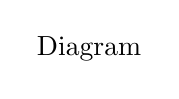
\begin{tikzpicture}
        \node {Diagram};
        \end{tikzpicture}
    \end{center}
\end{enumerate}
